\chapter{Models} \label{models}

In this chapter, we will build the models for range-Doppler map upsampling. According to the introduction in section \ref{overview of the state of the art}, there are mainly the following deep learning models, encoder-decoder architecture such as UNet architecture, Transformer model, \gls{cgan}, etc. Additionally, two layers are required in models, namely dimension processing layer and upsampling layer.

\section{Dimension processing layer} \label{dimension processing layer}
% padding or convolutional layer to make (129,32) to be (130, 32) or (128,32)
According to the \gls{rdp} introduced in section \ref{dataset loading} and the preprocessing types in section \ref{pre- and post-processing of the model inputs and outputs}, the input size of the model will be \texttt{(batch, \#samples//sampling\_rate//2+1, \#chirps//sampling\_rate, \#Frames or \#Frames*2)}. In order to explain the change of the shape easily and clearly, following will use the amplitude and phase representation type, batch size as 8, sampling rate as 2, the number of frames as 4 by default. In this combination, the shape of the low-resolution input will be \texttt{(8, 129, 32, 8)} and for high-resolution data as ground truth as \texttt{(8, 257, 64, 2)}. However, there is a problem with the current range dimension as an prime number. In the encoder-decoder architecture, it is difficult to choose a suitable stride for the current shape of the range axis because multiple times of the downsampling and upsampling layers will be performed. For the \gls{swin} Transformer, the current shape of range axis is also a troublesome size since the data needs to be split into multiple patches. Except the \gls{dp}-\gls{tf} Transformer model, since it calculates self-attention along the range and velocity axes separately, the problem of dimension does not need to be considered as well as our basic \gls{cnn} model, because it will not downsample the data.

There are three solutions for dimension processing layer. The first is that only in the case of \gls{dp}-\gls{tf} Transformer model and the basic \gls{cnn} model, it's possible to skip the additional dimension processing layer, and the model directly learns based on the input shape, but also ensure that there is no other downsampling process in the \gls{dp}-\gls{tf} Transformer model. In this case, since the model will perform an upsampling operation at the end, the dimension will become \texttt{(8, 258, 64, 2)}, so a cropping is required to select only the first 257 samples along the range axis.

Another option is that for models that need multiple downsampling layers such as in the encoder-decoder structure, it is more convenient when the range-Doppler map shape is in the power of 2, so the solution is to perform a convolutional layer along the range dimension, which uses a stride of 1 and the kernel size is set as \texttt{(2, 1)}, so that the input dimension of the model becomes \texttt{(8, 128, 32, 8)}. After passing through the model and subsequent upsampling layer, its dimension goes to \texttt{(8, 256, 64, 2)}. Therefore, there is always one less value in the range dimension. Then the transposed convolutional layer is needed, and also chosen stride as 1 and kernel size as \texttt{(2, 1)} to make its shape the same as ground truth.

However, while applying the convolutional layer according to the second option, the reduction in one dimension means that information may be lost. In order to alleviate this problem, the third solution is padding. By filling a row of 0 values along the range dimension, it will not lose input information and can become an even number, that is, the input becomes \texttt{(8, 130, 32, 8)}. Meanwhile, since it is not a power of 2, the downsampling layer can be performed only once in the model at most. In this case, after the final upsampling layer, the size of the output will be \texttt{(8, 260, 64, 2)}. There are extra \texttt{(2*sampling\_rate - 1)} samples in the range dimension, but since it was initially filled with 0, directly discarding this part will not cause information loss, that is, taking the values before the last \texttt{(2*sampling\_rate - 1)} dimension.

In summary, according to the input data representation, logarithm, normalization type as well as the dimension processing type, the preprocessing block can be combined with six forms as shown in Figure \ref{preprocessing_block}. The corresponding postprocessing module has six forms as well, illustrated in Figure \ref{postprocessing_block}. The green part in the preprocessing block is the input data that the model starts to process, while the red part in the postprocessing block is the output of the model for calculating the training loss with the ground truth.

\begin{figure}
	\centering
	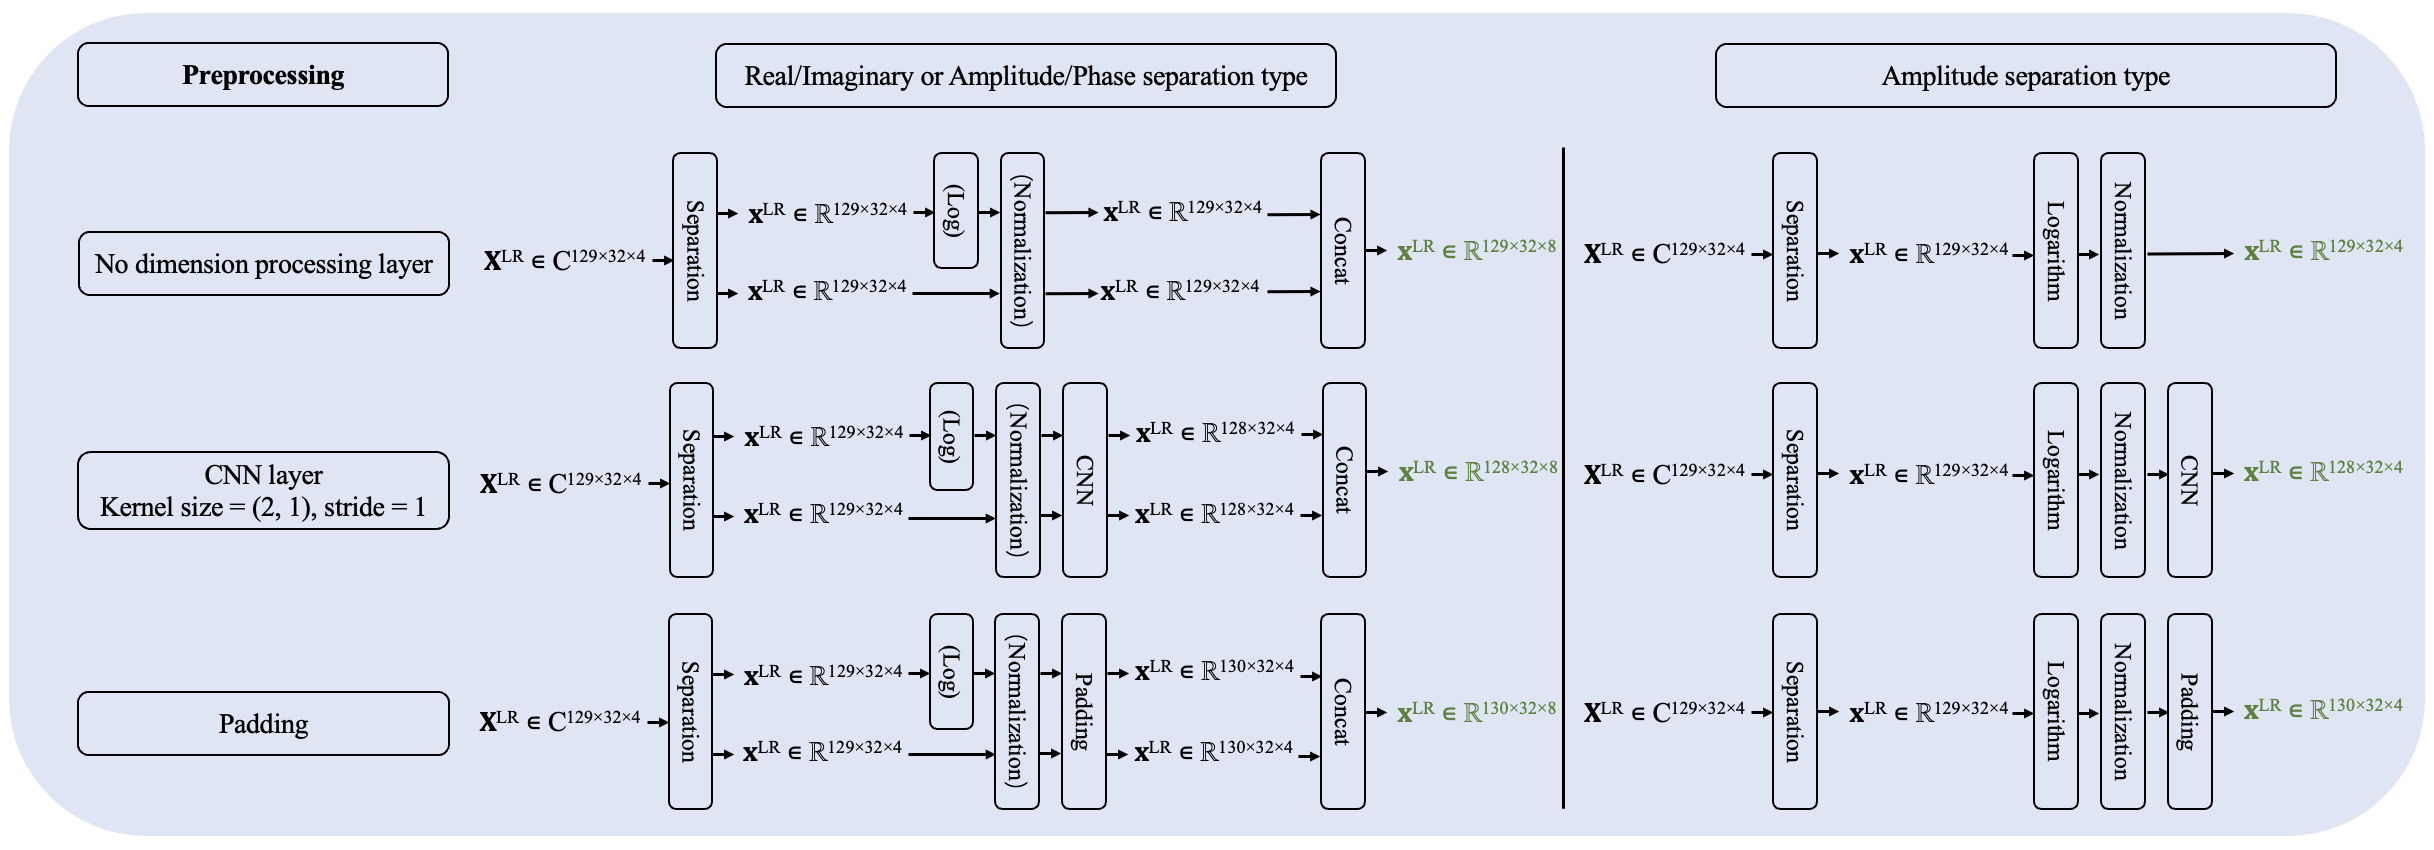
\includegraphics[scale=.45]{thesis/figures/preprocessing_block.png}
	\caption{Preprocessing block in the case of the number of frames as 4, where logarithm and normalization are not used in real and imaginary representation type and the green represents the model inputs.}
	\label{preprocessing_block}
\end{figure}

\begin{figure}
	\centering
	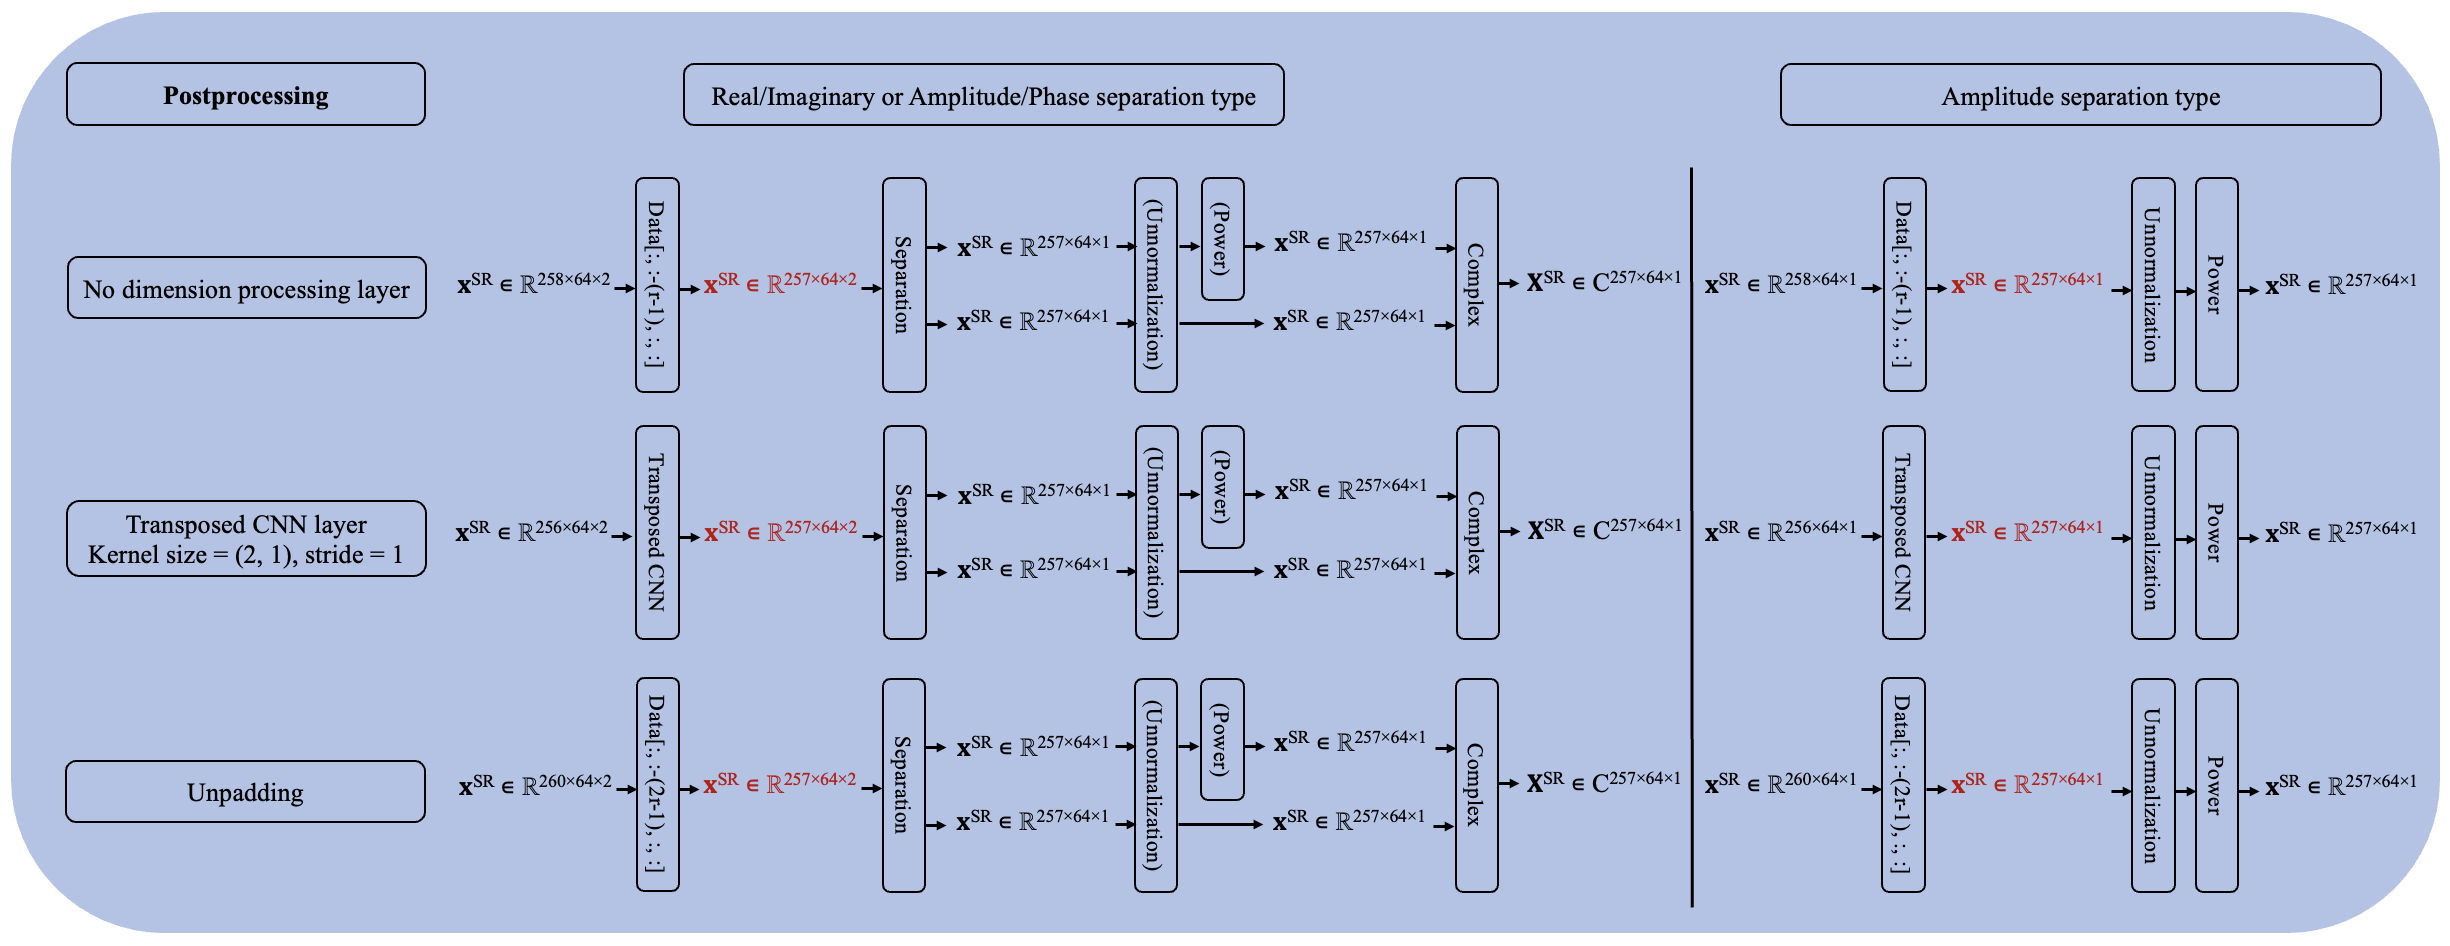
\includegraphics[scale=.42]{thesis/figures/postprocessing_block.png}
	\caption{Postprocessing block in the case of the number of frames as 4, where unnormalization and power of 10.0 are not used in real and imaginary representation type, the red represents the model outputs to calculate the training loss and r is the resample rate.}
	\label{postprocessing_block}
\end{figure}

\section{Upsampling layer} \label{upsampling layer}
% Transposed convolutional layer or Shuffle pixel
Before performing the upsampling layer, it's necessary to determine the times of upsampling layers required. Since the upsampling functions in TensorFlow or PyTorch usually doubles the resolution each time, the upsampling rate prefers to be a power of 2, so the times of upsampling operations in our case can be determined to be logarithmic sampling rate with the base as 2.

A common layer for upsampling is the transposed convolutional layer, whose operation is logically equivalent to the reverse convolutional layer as shown in Figure \ref{view of a transposed cnn layer}, but these two are not their respective inverse, that is, the transposed convolutional layer can not completely restore the range-Doppler map back to the original one before the convolutional layer. The shape relationship between the input and output of the transposed convolutional layer is
\begin{equation}
    \centering
    o = (i - 1) * s + k - 2 * p,
\end{equation}

where $s$ represents stride, $k$ is the kernel size, $p$ denotes the padding size, $i$ and $o$ are the shape of input and output, respectively.

\begin{figure}
	\centering
	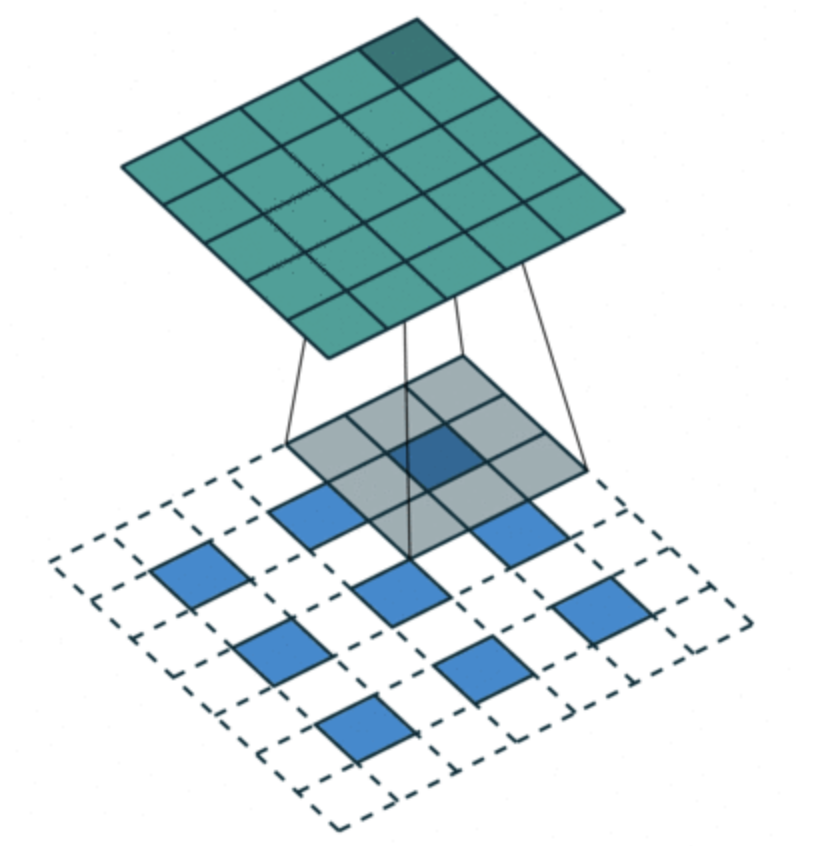
\includegraphics[scale=.45]{thesis/figures/transposed_cnn.png}
	\caption{View of the transposed convolutional layer in the case of the stride as 2, padding as 1 and kernel size as 3, where the blue is input and the green is output \cite{vdumoulin_vdumoulinconv_arithmetic_2025}.}
	\label{view of a transposed cnn layer}
\end{figure}

TensorFlow has a built-in transposed convolutional module. To facilitate upsampling, there are two options in the padding parameter, either valid or same. When same is selected, upsampling will be performed according to the stride value. Furthermore, each time the transposed convolutional layer is used, it will pass through the additional layer normalization and \gls{relu} activation layers as the other paper \cite{hinderer_blind_2022} did, which makes the training process more stable and converges faster as well as preventing the gradient explosion.

Another upsampling method is called pixel shuffle approach, also known as sub-pixel convolution or depth to space method, etc., proposed by Shi et al \cite{shi_real-time_2016}. As shown in Figure \ref{view of the pixel shuffle}, the principle is that the input data is processed by a series of hidden layers in the model, data of the shape \texttt{(N, C $\times$ r\textsuperscript{2}, H, W)} is obtained, where r denotes the resampling rate and all of the numbers are positive integers. Upsampling is achieved by splitting the size of \texttt{r\textsuperscript{2}} in depth and expanding its value into the dimensions of spaces, namely \texttt{H} and \texttt{W}.

There are two main benefits of pixel shuffle approach. Firstly, the pixel shuffle method does not require any other parameters, which can reduce the number of parameters and computational complexity compared to the transposed convolutional layer \cite{shi_is_nodate}. On the other hand, according to the paper from Odena, etc., one reason for the checkerboard effect is that the transposed convolutional layer causes overlapping, while the lack of overlapping in the method of pixel shuffle approach can mitigate this problem to a certain extent \cite{odena_deconvolution_2016}.

\begin{figure}
	\centering
	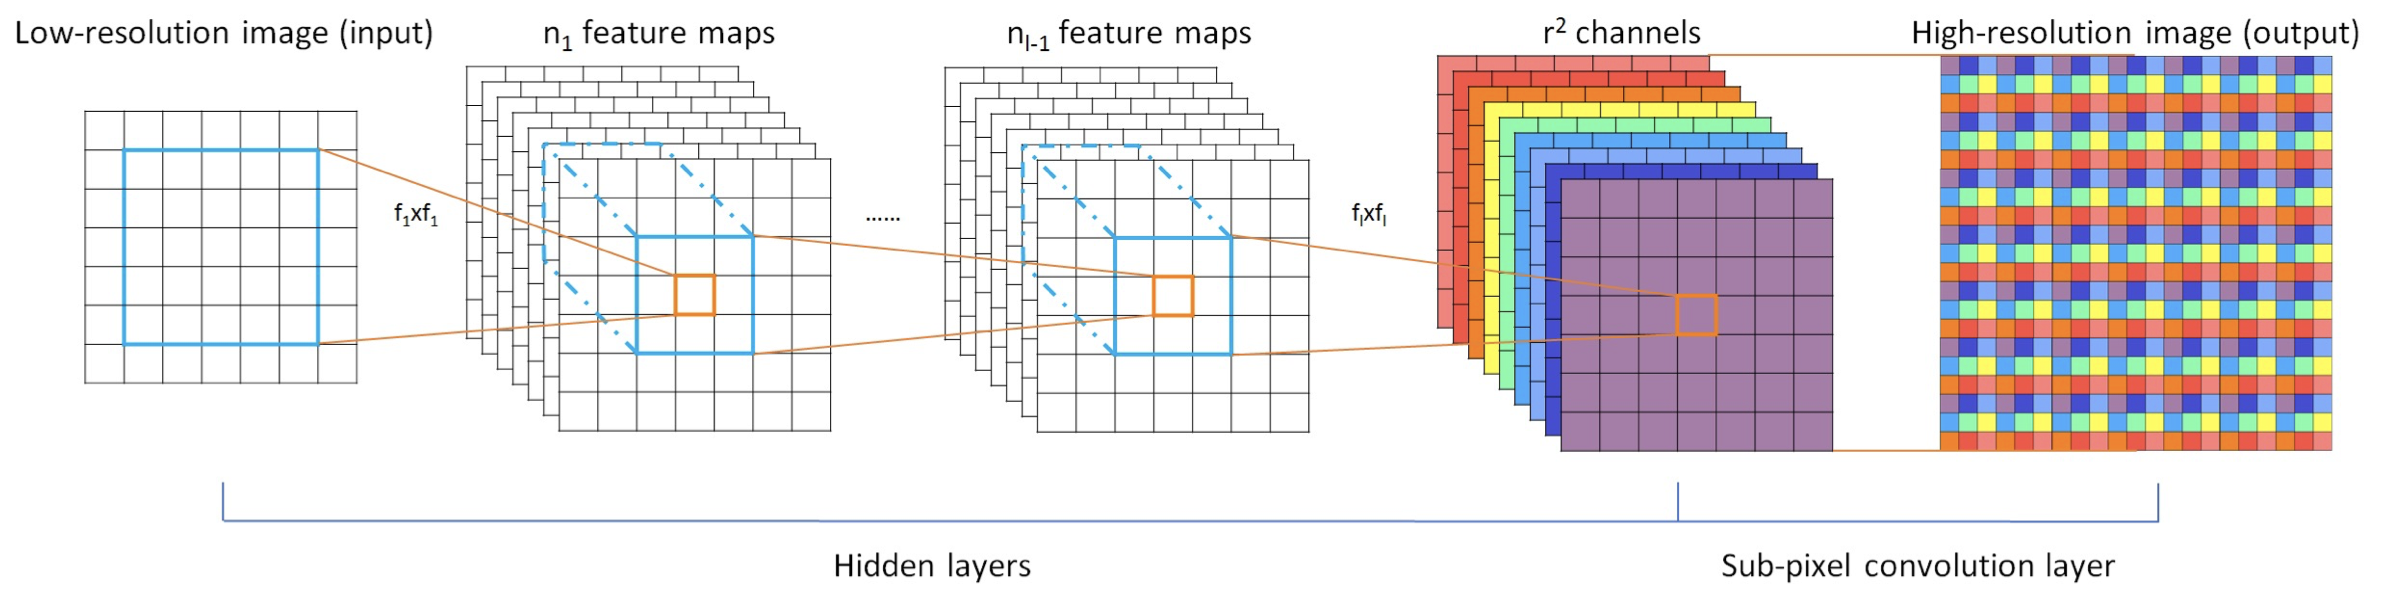
\includegraphics[scale=.35]{thesis/figures/pixelShuffle.png}
	\caption{View of the pixel shuffle approach, where r denotes the resample rate \cite{shi_real-time_2016}.}
	\label{view of the pixel shuffle}
\end{figure}

\section{Interpolation} \label{interpolation}
As a method that does not require any parameters and training process, the interpolation method can be used as a baseline in the range-Doppler upsampling task. Its principle is to interpolate a value in the middle according to the values of the surrounding points. Figure \ref{interpolation model} shows the interpolation model built in this thesis, which has two forms, Figure \ref{interpolation model left} and Figure \ref{interpolation model right}, according to the input data representation.

\begin{figure}
    \centering
    \hspace{-0.4cm}
    \begin{subfigure}{0.59\textwidth}
        \centering
        \adjustbox{height=12cm}{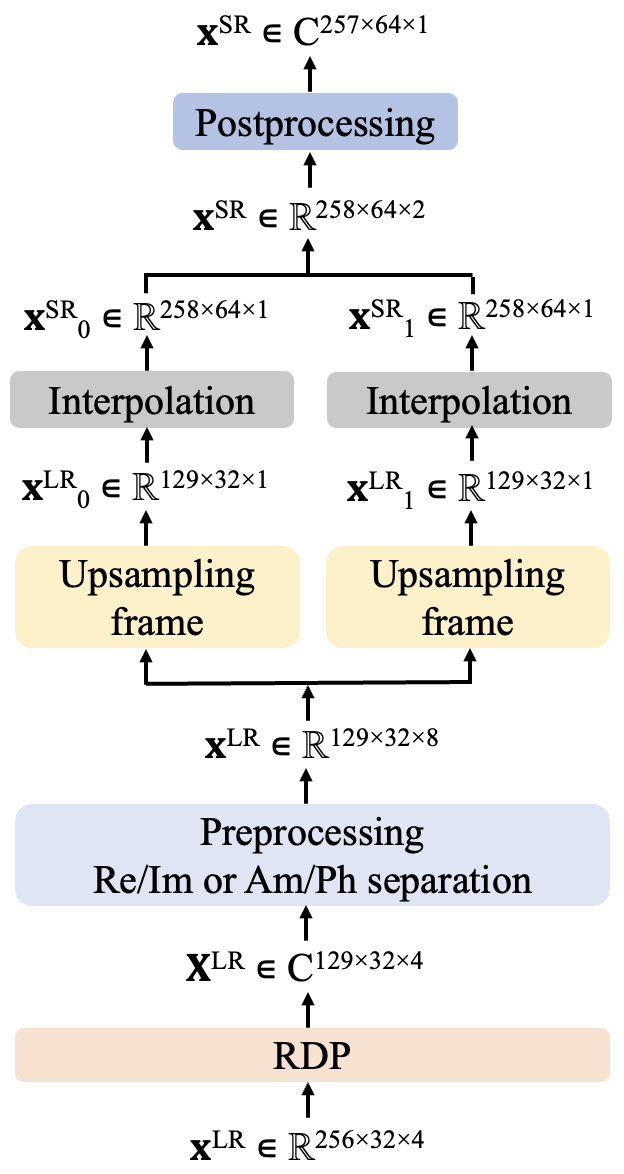
\includegraphics[scale=.25]{thesis/figures/interpolation_left.png}}
        \caption{Interpolation model with the real and imaginary or amplitude and phase representation types.}
        \label{interpolation model left}
    \end{subfigure}
    \begin{subfigure}{0.39\textwidth}
        \centering
        \adjustbox{height=12cm}{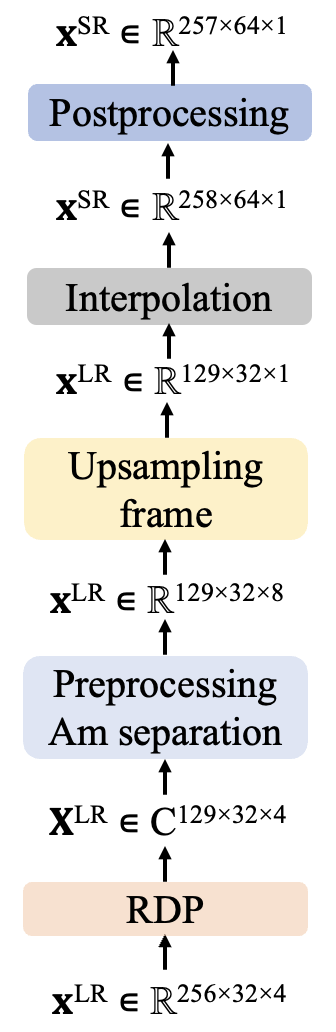
\includegraphics[scale=.25]{thesis/figures/interpolation_right.png}}
        \caption{Interpolation model with the amplitude representation type.}
        \label{interpolation model right}
    \end{subfigure}
    \caption{Interpolation models in terms of the representation types, in the case of the downsampling rate as 2 and the number of frames as 4.}
	\label{interpolation model}
\end{figure}

Assuming the same parameters as in section \ref{dimension processing layer} are used, that is, the batch size is set as 8, the data resampling rate is 2, and the number of frames is 4, the shape of the input is \texttt{(8, 129, 32, 8)} in the case of the real and imaginary or amplitude and phase representation types after preprocessing block. Since the interpolation method has no parameters and training process, it will directly process the low-resolution range-Doppler map which is going to be upsampled. According to the order of the number of frames in section \ref{dataset loading} and the input data representation mentioned in section \ref{pre- and post-processing of the model inputs and outputs}, the last dimension of the real part or the amplitude part $\text{x}^{\text{LR}}_0$ and the last dimension of the imaginary part or the phase part $\text{x}^{\text{LR}}_1$ are the data that need to be upsampled, so only these two frames are taken out.

For the interpolation process, TensorFlow provides many approaches. By default, bilinear interpolation is used in this model, as illustrated in Figure \ref{bilinear interpolation}, which is calculated based on the distance from the surrounding four points, namely
\begin{figure}
	\centering
	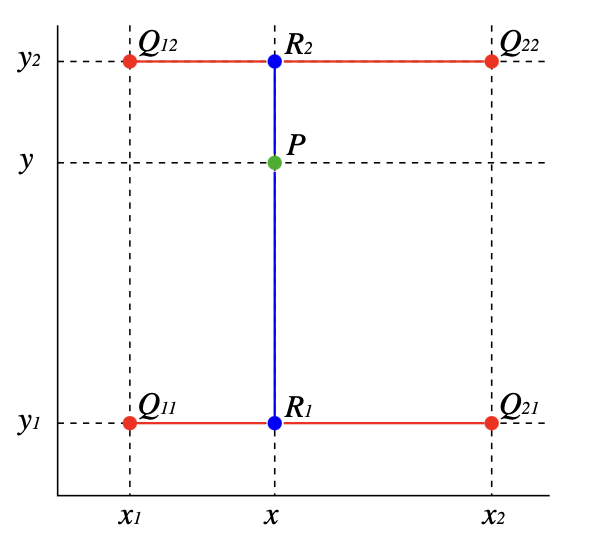
\includegraphics[scale=.7]{thesis/figures/bilinear.png}
	\caption{Bilinear interpolation, where $P$ is the interpolated point and $Q$s are the surrounding points \cite{noauthor_bilinear_2025}.}
	\label{bilinear interpolation}
\end{figure}

\begin{equation}
    \centering
    f(x, y) = \frac{1}{(x_2 - x_1)(y_2 - y_1)}
    \begin{bmatrix}
    x_2 - x & x - x_1
    \end{bmatrix}
    \begin{bmatrix}
    f(Q_{11}) & f(Q_{12}) \\
    f(Q_{21}) & f(Q_{22})
    \end{bmatrix}
    \begin{bmatrix}
    y_2 - y \\
    y - y_1
    \end{bmatrix},
\end{equation}

where $f(x, y)$ is the interpolation value at the point $(x, y)$. Furthermore, the default upsampling rate is 2 each time, so the sampling rate should be a power of 2. The model will be postprocessed according to the value of the resampling rate and as mentioned in section \ref{dimension processing layer} to make it the same size as the ground truth after stacking along the last dimension.

\section{CNN model} \label{cnn model}
Compared with the bilinear interpolation model, the most common model for image processing is the \glsfirst{cnn}. We introduced a relatively basic \gls{cnn} model, which does not downsample the data and performs the upsampling operation after one specified convolutional layer. The overview of the \gls{cnn} model is shown in Figure \ref{cnn model structure}.

\begin{figure}
	\centering
	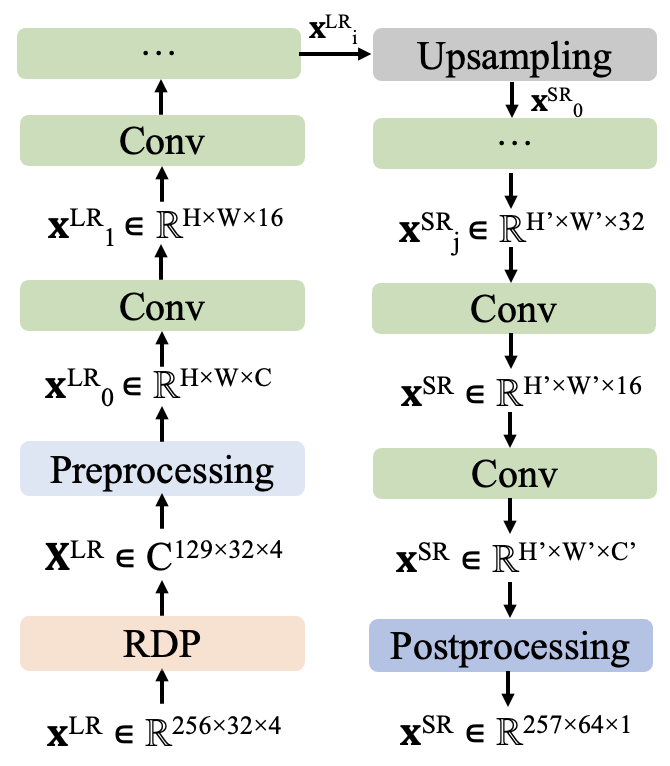
\includegraphics[scale=.63]{thesis/figures/cnn_simple.png}
	\caption{CNN model, where the channel, height and width are depending on the processing methods.}
	\label{cnn model structure}
\end{figure}

As shown, since the preprocessing is a combination of representation, dimension processing, logarithm and normalization types, the height \texttt{H} and width \texttt{W} depend on the selected dimension processing type, while the channel \texttt{C} and \texttt{C'} depend on the input data representation. The value of \texttt{C} can be 4 or 8, and then enters the convolutional layers. In this model, two parameters are set to facilitate the change of model scale, namely the neuron list and upsampling layer index. The neuron list represents a list of the channel values in the case of stride as 1, and the upsampling layer index indicates the position of the convolutional layer after which the upsampling layer is performed. Similarly, \texttt{H'} and \texttt{W'} are the sizes of the range-Doppler map after upsampling, which are also up to the dimension processing type, and are then converted into the same shape as the ground truth while postprocessing. The process can be written as

\begin{equation}
    \centering
    \text{x}^{\text{LR}}_i = \text{Conv2D}^{i}(\text{x}^{\text{LR}}_0),
\end{equation}

where $i$ is the upsampling layer index with the upsampling operation

\begin{equation}
    \centering
    \text{x}^{\text{SR}}_0 = \text{Upsampling}(\text{x}^{\text{LR}}_i),
\end{equation}

then the final super-resolution data after $j$ times convolutional layers is

\begin{equation}
    \centering
    \text{x}^{\text{SR}} = \text{Conv2D}(\text{Conv2D}^{j}(\text{x}^{\text{SR}}_0)).
\end{equation}

\begin{figure}[t]
	\centering
	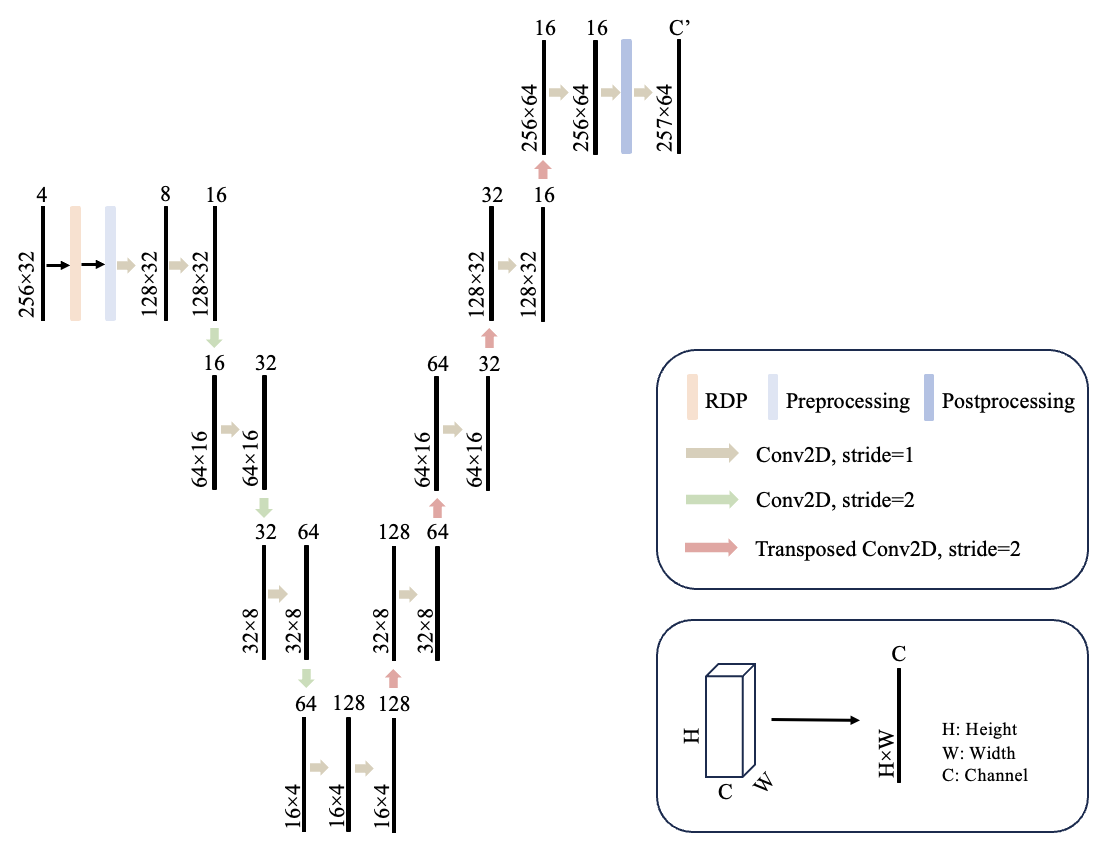
\includegraphics[scale=.8]{thesis/figures/unet_model.png}
	\caption{UNet model}
	\label{unet model}
\end{figure}

\section{UNet architecture} \label{u-net architecture}
As mentioned in section \ref{overview of the state of the art}, the encoder-decoder structure is very common for the upsampling task in deep learning. During the encoder process, the model will do the downsampling operations and learn important features from the data, and then perform multiple upsampling layers based on the learned information. The most common model is the UNet model, so we built it based on the convolutional layers with the stride as 2. Compared with the \gls{cnn} model in section \ref{cnn model}, the downsampling process may cause information loss. Inspired by the paper \cite{prabhakara_high_2023} from Akarsh et al., by adding residual connections between the encoder and decoder parts, the information loss problem is alleviated. Therefore, in this section, there will be two parts, namely basic UNet model and UNet concat model.

\subsection{UNet model} \label{UNet model subsection}
The overview of the UNet model is illustrated in Figure \ref{unet model}. Since there are multiple downsampling operations in the UNet model and the default downsampling rate is 2, the data size in height and width should be the power of 2. Therefore, the dimension processing layer is determined as the convolutional layer approach in most cases. Otherwise, only once downsampling can be done if using padding. Meanwhile, due to the representation type, the channel would be either 4 or 8, and while passing through the first convolutional layer, this dimension is uniformly converted to 8.

In the UNet model, four times downsamplings are performed by default, and different numbers of upsampling layers are performed according to the resampling rate. When the resampling rate is 2, five times upsampling are performed. Before each upsampling layer, a convolutional layer with a stride of 1 is performed, and the number of channels is meanwhile modified. The upsampling operation uses the transposed convolutional layer by default. In postprocessing part, the corresponding unit parameters are set according to the data representation type.

\subsection{UNet concat model} \label{UNet concat model subsection}
As mentioned above, to mitigate the information loss during downsamping operations, in UNet concat model the upsampling data will be concatenated with the downsampled data, as shown in Figure \ref{unet_concat model}. 

\begin{figure}
	\centering
	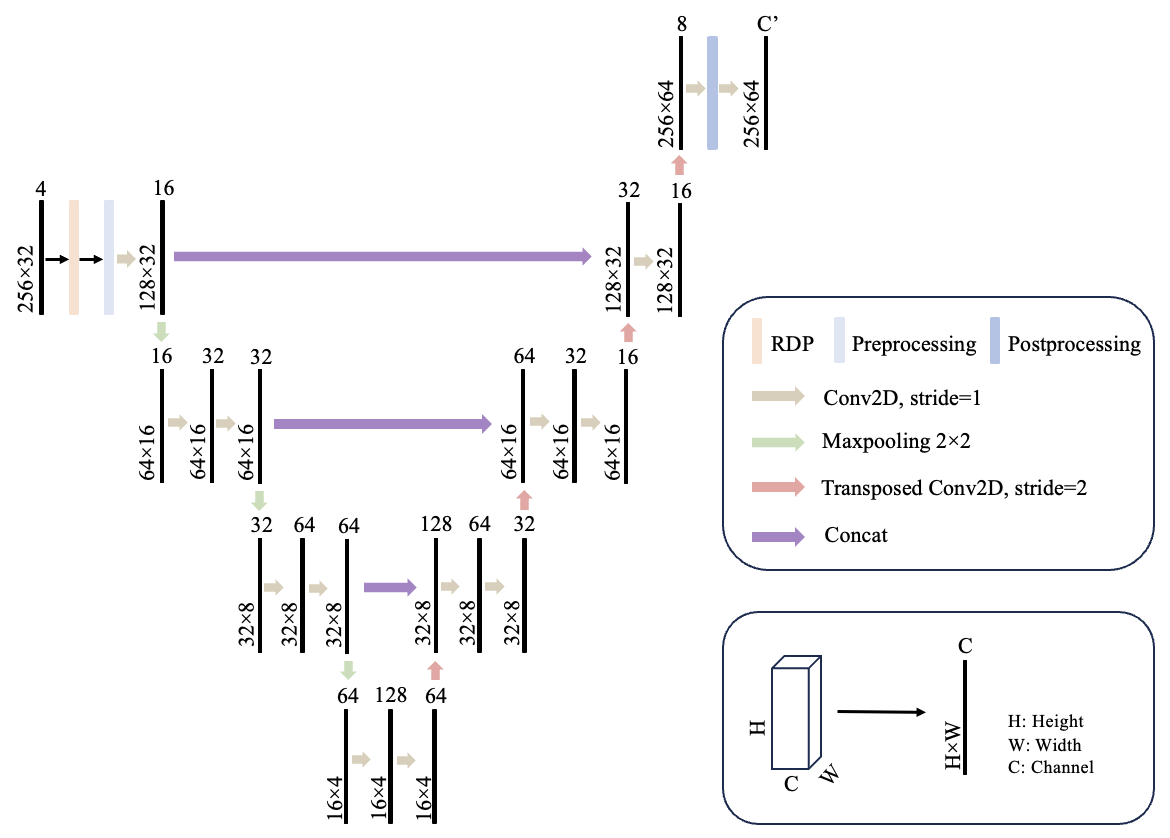
\includegraphics[scale=.75]{thesis/figures/unet_concat.png}
	\caption{UNet concat model}
	\label{unet_concat model}
\end{figure}

Compared with the UNet model in section \ref{UNet model subsection}, the UNet concat model has the following four main differences. First, the encoder part passes through two convolutional layers with a stride of 1 instead of just one layer. Moreover, in the decoder part, the UNet model only passes through the convolutional layer once to reduce the channel before the upsampling layer, while UNet concat model passes through two convolutional layers and reduces the channel dimension twice. The UNet model uses a convolutional layer with a stride of 2 for downsampling, while UNet concat model uses a 2$\times$2 maxpooling layer. In addition, during each upsampling process, the data is concatenated with the corresponding downsampled data of the same size along the channel dimension.

\section{DP-TF Transformer architecture} \label{dp-tf transformer architecture}
As mentioned in section \ref{overview of the state of the art}, Transformer is a state-of-the-art model in the task of data upsampling. It uses the self-attention mechanism to learn the similarities and relationships between different blocks. In the range-Doppler map, the objects have a certain correlation in the dimension of the range and velocity related to the radar. Furthermore, the consecutive motion can also bring some additional motion information as well. In this model, it will mainly focus on the division along the two dimensions of range and velocity.

Figure \ref{dp-tf_transformer_architecture} shows the overall structure of this model. Compared with the models mentioned previously, it mainly has three different blocks: feature extractor, feature Transformer, and reconstruction. According to \cite{hinderer_blind_2022}, feature extractor is equivalent as an encoder, but since additional downsampling may cause information loss, the stride of the convolutional layer will be set as 1 in the featur extractor. The reconstruction is equivalent as the decoder, and the additional upsampling is performed according to the resample rate.

\begin{figure}
	\centering
	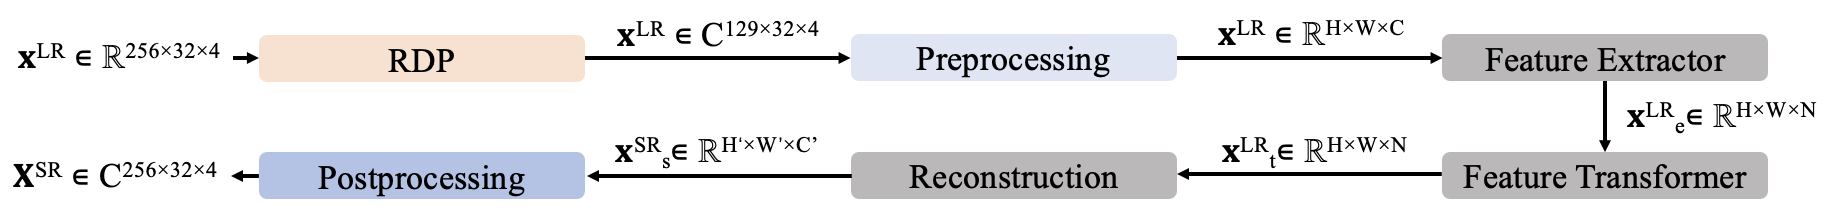
\includegraphics[scale=.5]{thesis/figures/dp-tf_transformer_architecture.png}
	\caption{DP-TF Transformer architecture, adapted from \cite{hinderer_blind_2022}.}
	\label{dp-tf_transformer_architecture}
\end{figure}

\begin{spacing}{1.5}
\textbf{\large{Feature Extractor}}
\end{spacing}

The feature extractor mainly includes two steps. The first step will perform a separable convolutional layer and a \gls{ln} to obtain an intermediate feature extractor representation $\mathrm{x^{LR}_{e1}}$ expressed as

\begin{equation}
    \centering
    \mathrm{x^{LR}_{e1} = LN(SeparableConv2D(x^{LR}))},
    \label{first separable conv2D equation in feature extractor}
\end{equation}

where $\mathrm{x^{LR}_{e1} \in \mathbb{R}^{H\times W\times N}}$ and H, W and N represent the height, width and channel size, respectively. In the second step, a SeparableConv2D layer and a \gls{ln} are also performed, where SeparableConv2D layer still sets stride as 1 and does not perform downsampling in our case. In addition, a \gls{relu} activation function layer will be used, written as

\begin{equation}
    \centering
    \mathrm{x^{LR}_{e2} = ReLU(LN(SeparableConv2D(x^{LR}_{e1})))},
    \label{second conv block after first conv in feature extractor}
\end{equation}

where $\mathrm{x^{LR}_{e2} \in \mathbb{R}^{H\times W\times N}}$ still. According to the paper, another convolutional layer is used. Although the downsampling operation is not performed in our case, we can still keep it. The output of the feature extractor can be written as

\begin{equation}
    \centering
    \mathrm{x^{LR}_{e} = LN(Conv2D(x^{LR}_{e2}))}.
    \label{third equation in feature extractor}
\end{equation}

\begin{spacing}{1.5}
\textbf{\large{Feature Transformer}}
\end{spacing}

The feature Transformer mainly includes three hierarchies, as shown in Figures \ref{feature_transformer_block}, \ref{dp_transformer_block}, and \ref{transformer_block}. Figure \ref{feature_transformer_block} shows the overall structure of the feature Transformer, Figure \ref{dp_transformer_block} shows the structure of the \gls{dp}-\gls{tf} Transformer block and the way to do the data segmentation, and Figure \ref{transformer_block} shows the structure of the \gls{te}.

\begin{figure}
	\centering
	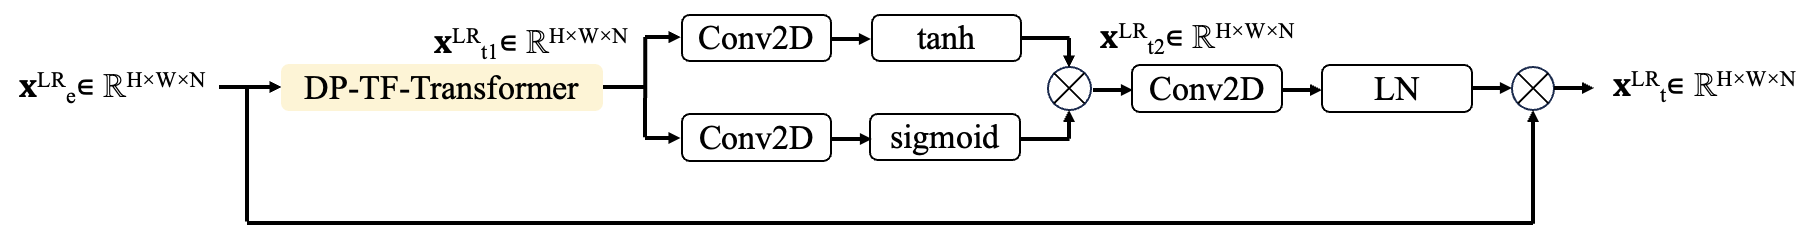
\includegraphics[scale=.48]{thesis/figures/feature_transformer_block.png}
	\caption{Feature Transformer block, adapted from \cite{hinderer_blind_2022}.}
	\label{feature_transformer_block}
\end{figure}

\begin{figure}
	\centering
	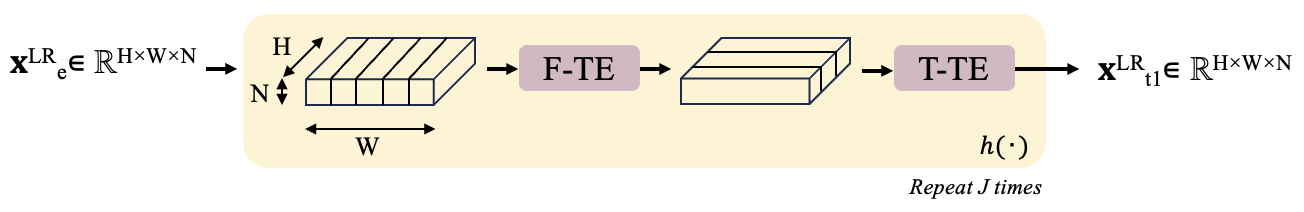
\includegraphics[scale=.66]{thesis/figures/dp_transformer_block.png}
	\caption{DP-TF Transformer block, adapted from \cite{hinderer_blind_2022}.}
	\label{dp_transformer_block}
\end{figure}

\begin{figure}
	\centering
	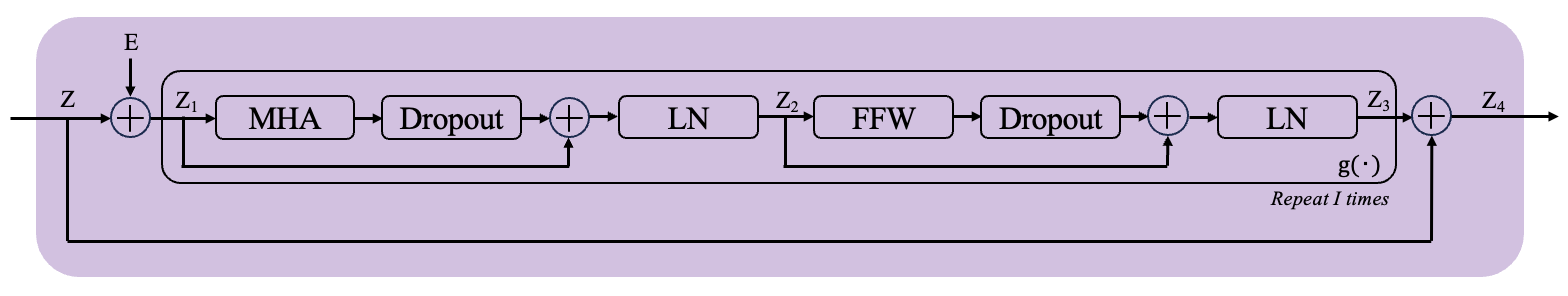
\includegraphics[scale=.55]{thesis/figures/transformer_block.png}
	\caption{TE block, adapted from \cite{hinderer_blind_2022}.}
	\label{transformer_block}
\end{figure}

In the first hierarchy of the feature Transformer, the data will be firstly operated by the \gls{dp}-\gls{tf} Transformer block. Subsequently, the output passes through the dual path which can be seen as a gating mechanism. Each path includes a convolutional layer and an activation function. The activation function as tanh keeps the main content into (-1, 1) while the other activation function uses sigmoid that leads the output into (0, 1). Then the two values are multiplied elementwise which is beneficial for remaining the useful information and discarding the feature with lower importance, namely
\begin{equation}
    \centering
    \mathrm{x^{LR}_{t2} = tanh(Conv2D(x^{LR}_{t1})) \circ sigmoid(Conv2D(x^{LR}_{t1}))}.
    \label{first equation in feature transformer}
\end{equation}

Furthermore, an additional convolutional layer and a layer normalization will be performed as well as a residual path, written as
\begin{equation}
    \centering
    \mathrm{x^{LR}_{t} = x^{LR}_{e} \circ LN(Conv2D(x^{LR}_{t2}))}.
    \label{second equation in feature transformer}
\end{equation}

In the second hierarchy, that is, in the \gls{dp}-\gls{tf} Transformer block, the data are divided along the range and velocity axes and each division has a \gls{te} block respectively, described as
\begin{equation}
    \centering
    \mathrm{x^{LR}_{t1}} = h^{j}\mathrm{(x^{LR}_{e})},
\end{equation}

where $h^{j}(\cdot)$ denotes $J$ times \gls{dp}-\gls{tf} Transformer block applications. Within the \gls{te} block, a sinusoidal positional encodings will be firstly added to the input as the representation of the order of the inputs, namely
\begin{equation}
    \centering
    \mathrm{Z_1 = Z + E},
\end{equation}

then a module $g(\cdot)$ as shown in Figure \ref{transformer_block} will be performed $I$ times on $\mathrm{Z_1}$ with a residual path with Z, written as
\begin{equation}
    \centering
    \mathrm{Z_4} = g^{I}\mathrm{(Z_1) + Z},
\end{equation}

where within this module, a multi-head attention block and a dropout layer will be performed on $\mathrm{Z_1}$, a residual path exists before the layer normalization, resulting in $\mathrm{Z_2}$
\begin{equation}
    \centering
    \mathrm{Z_2 = LN(Z_1 + Dropout(MHA(Z_1)))}.
\end{equation}

Moreover, another similar part will be performed, replace the MHA with a point-wise \gls{ffw} network, resulting in $\mathrm{Z_3}$
\begin{equation}
    \centering
    \mathrm{Z_3 = LN(Z_2 + Dropout(FFW(Z_2)))},
\end{equation}

where \gls{ffw} block contains two dense layers and a \gls{relu} activation function, that is,
\begin{equation}
    \centering
    \mathrm{Z'_2 = Dense(ReLU(Dense(Z_2)))},
    \label{ffw equation}
\end{equation}

\begin{spacing}{1.5}
\textbf{\large{Reconstruction}}
\end{spacing}

In the super-resolution data reconstruction, an upsampling layer will be performed firstly. If the transposed convolutional layer is used, it will combine with a layer normalization and a \gls{relu} activation function, namely
\begin{equation}
    \centering
    \mathrm{x^{SR}_{s1} = ReLU(LN(Conv2DTranspose(x^{LR}_t)))}.
    \label{separator1 equation}
\end{equation}

According to the input data representation, the unit of the last convolutional layer could be determined as either 1 or 2 with the linear activation, written as
\begin{equation}
    \centering
    \mathrm{x^{SR}_s = Conv2D(x^{SR}_{s1})}.
    \label{separator2 equation}
\end{equation}

\section{SwinIR Transformer architecture} \label{swinir transformer architecture}
According to \cite{liang_swinir_2021} mentioned in section \ref{overview of the state of the art}, in addition to dividing the data along the two dimensions of range and velocity, it can also be divided into multiple quadratic range velocity patches. The structure is shown in Figure \ref{swinir_architecture}, which mainly includes three parts: shallow feature extraction, deep feature extraction, and super-resolution image reconstruction.

\begin{figure}
	\centering
	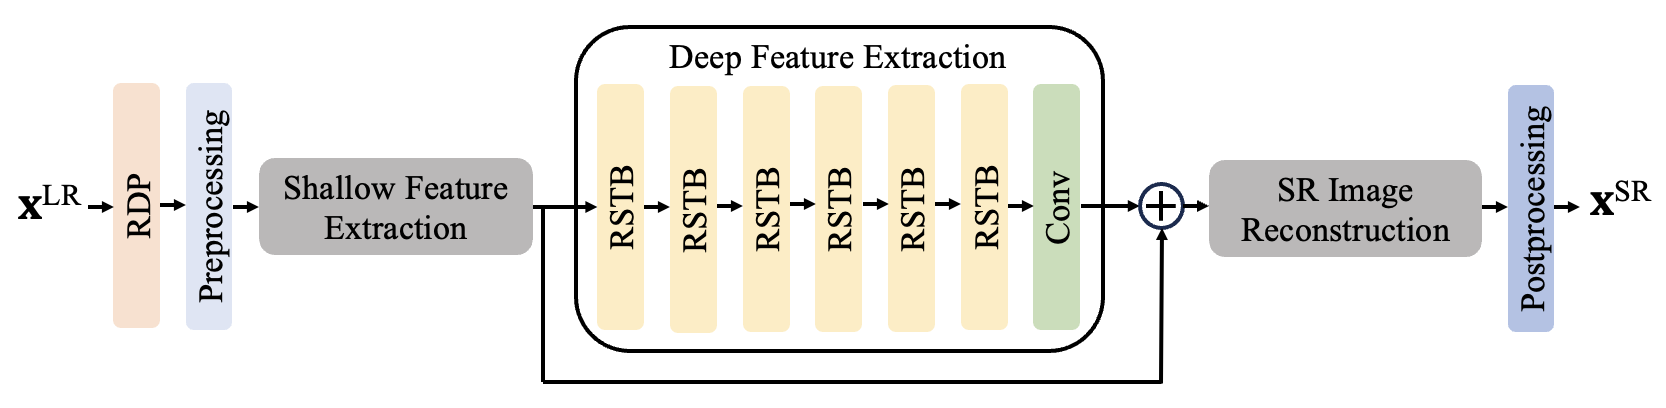
\includegraphics[scale=.53]{thesis/figures/swinir_architecture.png}
	\caption{SwinIR architecture, adapted from \cite{liang_swinir_2021}.}
	\label{swinir_architecture}
\end{figure}

In the paper, the \gls{swin} Transformer is used in the \gls{swinir} architecture, since we still have a \gls{dp}-\gls{tf} Transformer block, they can be combined as two models, namely SwinIR+Swin model and SwinIR+DP model.

\subsection{SwinIR+Swin model}

\begin{spacing}{1.5}
\textbf{\large{Shallow feature extraction}}
\end{spacing}

In the paper, the shallow feature extraction is seen as an encoder, which downsamples the data once. In order to mitigate the impact of information loss, a convolutional layer is still performed here but the stride is determined as 1, then the data size remains unchanged while only the channel is increased, namely
\begin{equation}
    \centering
    \mathrm{x^{LR}_s = Conv2D(x^{LR})}.
    \label{conv2D in shallow feature extraction equation}
\end{equation}

\begin{spacing}{1.5}
\textbf{\large{Deep feature extraction}}
\end{spacing}

In deep feature extraction, a dropout layer is performed first, then multiple \gls{rstb} and a convolutional layer are included, and the output of the deep feature extraction block is combined with the result of shallow feature extraction using the residual path, that is,
\begin{equation}
    \centering
    \text{x}^{\text{LR}}_\text{d} = \text{Conv2D}(\text{RSTB}^{J}(\text{Dropout}(\text{x}^{\text{LR}}_\text{s}))) + \text{x}^{\text{LR}}_\text{s},
    \label{first equation in deep feature extraction}
\end{equation}

where $J$ denotes the times of the \gls{rstb} applications. Figure \ref{rstb_block} illustrates the structure of the \gls{rstb}, where it contains multiple \gls{stl} blocks and a convolutional layer as well as the residual path, namely
\begin{equation}
    \centering
    \mathrm{{Z}_{R1}} = \text{Conv2D}(\text{STL}^{I}(\mathrm{Z_{R}})) + \mathrm{Z_{R}},
\end{equation}

where $I$ represents the times of the \gls{stl} applications. There are two parts inside the \gls{stl} block, one part includes a layer normalization, a \gls{msa} block as well as the residual part, described as
\begin{equation}
    \centering
    \mathrm{Z_{S1} = MSA(LN(Z_{S})) + Z_{S}},
\end{equation}

while another part contains a layer normalization, a \gls{mlp} and the residual path, namely
\begin{equation}
    \centering
    \mathrm{Z_{S2} = MLP(LN(Z_{S1})) + Z_{S1}}.
\end{equation}

In the \gls{mlp} block, five steps are carried out in sequence, namely dense layer, GeLU activation function, dropout layer, dense layer with linear activation function and dropout layer, denoted as
\begin{equation}
    \centering
    \mathrm{Z_{M1} = Dropout(GeLU(Dense(Z_{M})))},
    \label{mlp equation1}
\end{equation}

\begin{equation}
    \centering
    \mathrm{Z_{M2} = Dropout(Dense(Z_{M1}))}.
\end{equation}

\begin{figure}
    \centering
    \hspace{-0.4cm}
    \begin{subfigure}{0.49\textwidth}
        \centering
        \adjustbox{height=3.9cm}{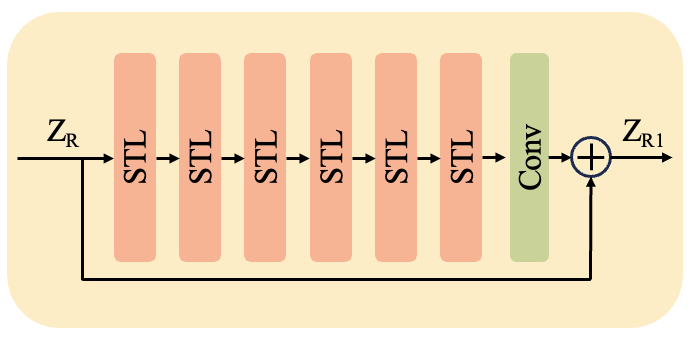
\includegraphics[scale=.24]{thesis/figures/rstb_block.png}}
        \caption{Structure of the \gls{rstb} block}
        \label{rstb_block}
    \end{subfigure}
    \begin{subfigure}{0.49\textwidth}
        \centering
        \adjustbox{height=3.75cm}{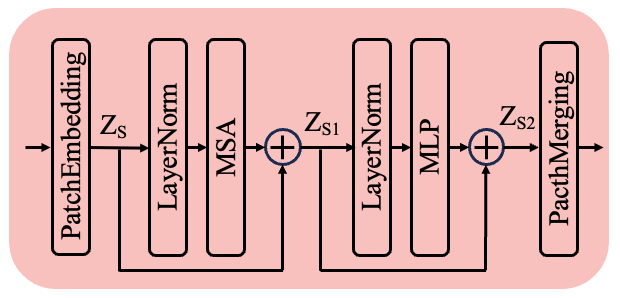
\includegraphics[scale=.24]{thesis/figures/stl_block.png}}
        \caption{Structure of the \gls{stl} block}
        \label{stl_block}
    \end{subfigure}
    \caption{The structure of \gls{rstb} and \gls{stl} blocks, adapted from \cite{liang_swinir_2021}.}
	\label{structure of the rstb and stl blocks}
\end{figure}

\begin{spacing}{1.5}
\textbf{\large{SR Image Reconstruction}}
\end{spacing}

The SR image reconstruction block includes three parts: the upsampling part as well as convolutional part before and after upsampling. There is a convolutional layer with the LeakyReLU activation function before the upsampling part, that is,
\begin{equation}
    \centering
    \mathrm{x^{LR}_{r} = LeakyReLU(Conv2D(x^{LR}_{d}))}.
\end{equation}

In the next step, the upsampling part is same as the reconstruction part in the section \ref{dp-tf transformer architecture}, namely the equation \ref{separator1 equation} and \ref{separator2 equation} resulting in $\mathrm{x^{SR}_{r1}}$ if using the transposed convolutional layer. After the upsampling part, another convolutional layer with the linear activation function is performed to make sure that the channel dimension of the output is according to the input data representation, namely the unit as either 1 or 2, written as
\begin{equation}
    \centering
    \mathrm{x^{SR}_r = Conv2D(x^{SR}_{r1})}.
\end{equation}

\subsection{SwinIR+DP model}
Combining with \gls{dp}-\gls{tf} Transformer block, the difference between SwinIR+Swin model is the \gls{stl} block. The structure of the \gls{stl} block as shown in Figure \ref{stl_block} can be replaced by the \gls{dp}-\gls{tf} Transformer block which is illustrated in Figure \ref{dp_transformer_block}.

\section{Comparison between the architectures} \label{comparison between the architecture}
According to all the models mentioned above, the differences between most models are relatively clear. For example, there is no downsampling process in the \gls{cnn} model. The difference between UNet and UNet concat models is mainly whether to combine the data of the encoder part with the corresponding decoder part. However, for the \gls{dp}-\gls{tf} Transformer model, the SwinIR+DP and SwinIR+Swin models, the data division is the main difference, but there are still some other small differences. Therefore, this section will focus on two parts, one is the difference between the \gls{dp}-\gls{tf} Transformer and \gls{swinir} architectures, and the other is the difference between the \gls{dp}-\gls{tf} and \gls{stl} Transformer blocks. The evaluation of this section will shown in the appendix.

\subsection{Differences between DP-TF and SwinIR Transformer architectures}
The main structures of the two architectures are very similar, both of which contain three parts: encoder, deep feature extraction, and decoder, so the differences will be listed in this order.

\begin{spacing}{1.5}
\textbf{\large{Encoder}}
\end{spacing}
They both have the encoder part, in \gls{dp}-\gls{tf} Transformer architecture it's called the feature extractor block, whereas in \gls{swinir} it's called shallow feature extraction.

\begin{enumerate}
    \item The feature extractor block of the \gls{dp}-\gls{tf} Transformer architecture uses the separable convolutional layer while in \gls{swinir} the normal convolutional layer, as written in formulas \ref{first separable conv2D equation in feature extractor} and \ref{conv2D in shallow feature extraction equation}.
    \item After the first separable convolutional layer, there's another layer normalization in the \gls{dp}-\gls{tf} Transformer architecture.
    \item In the feature extractor block, \gls{dp}-\gls{tf} Transformer architecture has an additional convolutional layer, layer normalization as well as the ReLU activation function layer, namely formula \ref{second conv block after first conv in feature extractor}.
\end{enumerate}

\begin{spacing}{1.5}
\textbf{\large{Transformer blocks}}
\end{spacing}
Both of the architectures use some blocks to loop the Transformer modules, feature Transformer in \gls{dp}-\gls{tf} architecture and deep feature extraction in \gls{swinir} architecture.

\begin{enumerate}[start=4]
    \item \gls{swinir} architecture has a dropout layer before the first \gls{rstb} block in the deep feature extraction block, as shown in formula \ref{first equation in deep feature extraction}.
    \item Before the \gls{dp}-\gls{tf} Transformer block in \gls{dp} architecture, another convolutional layer with layer normalization exists, that is, formula \ref{third equation in feature extractor}.
    \item \gls{swinir} architecture doesn't use dual path after the \gls{rstb} blocks as in \gls{dp}-\gls{tf} Transformer architecture shown in Figure \ref{feature_transformer_block}.
    \item \gls{swinir} sets a convolutional layer after \gls{rstb} and \gls{stl} blocks, whereas \gls{dp}-\gls{tf} architecture has convolutional layer with layer normalization after the dual path, i.e. in Figures \ref{swinir_architecture}, \ref{rstb_block} and \ref{feature_transformer_block}.
    \item In \gls{dp}-\gls{tf} Transformer architecture, the residual path in the feature Transformer uses multiply operation rather than adding, namely formula \ref{second equation in feature transformer}.
    \item \gls{swinir} architecture has an overall residual path, combining the output of the shallow feature extraction with the output of the deep feature extraction, as shown in Figure \ref{swinir_architecture}.
\end{enumerate}

\begin{spacing}{1.5}
\textbf{\large{Decoder}}
\end{spacing}
The decoder part is called reconstruction in \gls{dp}-\gls{tf} Transformer architecture while called SR image reconstruction in \gls{swinir} architecture. In this part, they don't have many differences, only one is that the kernel size in reconstruction is set as 1 by default while in SR image reconstruction block as a hyperparameter.

\subsection{Differences between DP-TF and Swin Transformer blocks}
Compared with the Transformer block as shown in Figure \ref{transformer_block} and \ref{stl_block}, some differences are existing as following:

\begin{enumerate}[start=10]
    \item According to the formulas \ref{ffw equation} and \ref{mlp equation1}, the activation functions are different, \gls{relu} in \gls{ffw} block while GeLU in \gls{mlp} block.
    \item The order of the items in the \gls{te} and \gls{stl} blocks is different.
    \item The residual path in both Transformer blocks are not the same, in \gls{swin} Transformer block there's no overall residual path but the layer normalization is inside the residual paths while in \gls{dp}-\gls{tf} Transformer block the layer normalization is after each residual paths.
\end{enumerate}

\section{cGAN architecture} \label{cgan architecture}
As mentioned in section \ref{overview of the state of the art}, some image upsampling papers use \gls{cgan} model. Although it may cause some loss functions to increase in value, the generator and discriminator can be trained mutually and the super-resolution range-Doppler map could be visually better.

\subsection{Generator} \label{generator}
In our task, generator refers to the model that learns from the source domain input as the low-resolution range-Doppler maps and generates super-resolution range-Doppler maps. All the models mentioned above can be used as the generator, but in order to reduce the complexity of combinations and evaluations, in the section \ref{models comparisons}, we will compare the performance of different models under various evaluation loss functions and select the good one as the generator.

\subsection{Discriminator} \label{discriminator}
The task of the discriminator is to distinguish between super-resolution range-Doppler map and truly high-resolution range-Doppler map. Through the learning and supervision of the discriminator, the output of the generator could look more realistic. The output of the discriminator will be a probability value, indicating the probability that the input data could be the truly high-resolution data. For the discriminator, its goal is to have the output probability approaching 0 when the input is the super-resolution data, and approaching 1 with the high-resolution data as input.

For the discriminator, we build two structures, depending on whether the input contains the corresponding low-resolution range-Doppler maps, as illustrated in Figure \ref{structures of the discriminator}. The discriminator in Keras tutorial \cite{team_keras_cgan} uses both source domain input as the low-resolution range-Doppler map and the target domain input as the super- or high-resolution range-Doppler map, while in some papers, such as \cite{ledig_photo-realistic_2017}, the low-resolution range-Doppler map is not input as additional information.

The structures of both discriminators are to obtain a probability value after a series of downsampling operations, and then performed by a dense layer with sigmoid as the activation function. The difference is that there is an extra concatenating operation in Figure \ref{discriminator inclusive low resolution image as input}. Furthermore, as the range-Doppler maps are given into the discriminator in the first step, the dimension processing type is determined as the convolutional layer, since the height is an odd value and the later convolutional layers set stride as 2 as well as the batch normalization layer and leaky \gls{relu} activation function, shown in Figure \ref{downsample block in discriminator}.

\begin{figure}
    \centering
    \hspace{-0.4cm}
    \begin{subfigure}{0.49\textwidth}
        \centering
        \adjustbox{height=7cm}{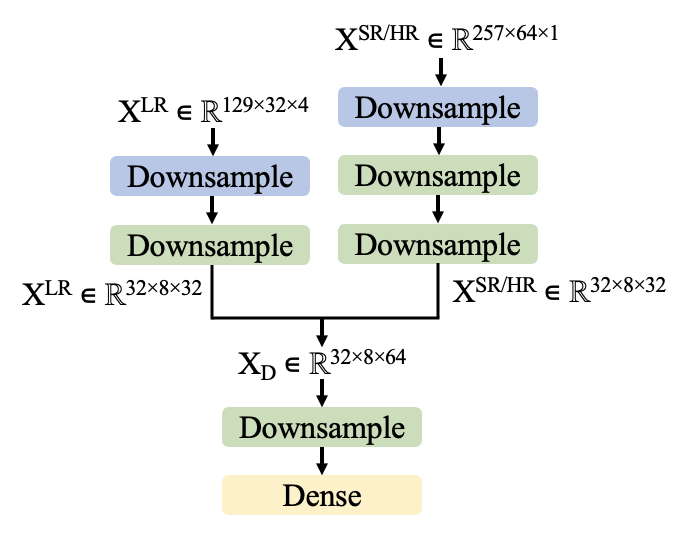
\includegraphics[scale=.24]{thesis/figures/discriminator_left.png}}
        \caption{Conditional discriminator inclusive low-resolution range-Doppler map as condition}
        \label{discriminator inclusive low resolution image as input}
    \end{subfigure}
    \begin{subfigure}{0.49\textwidth}
        \centering
        \adjustbox{height=7cm}{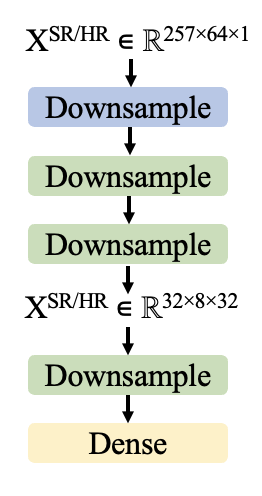
\includegraphics[scale=.24]{thesis/figures/discriminator_right.png}}
        \caption{Discriminator exclusive low-resolution range-Doppler map as input}
        \label{discriminator exclusive low resolution image as input}
    \end{subfigure}
    \caption{The structures of the discriminator in terms of the input}
	\label{structures of the discriminator}
\end{figure}

\begin{figure}
	\centering
	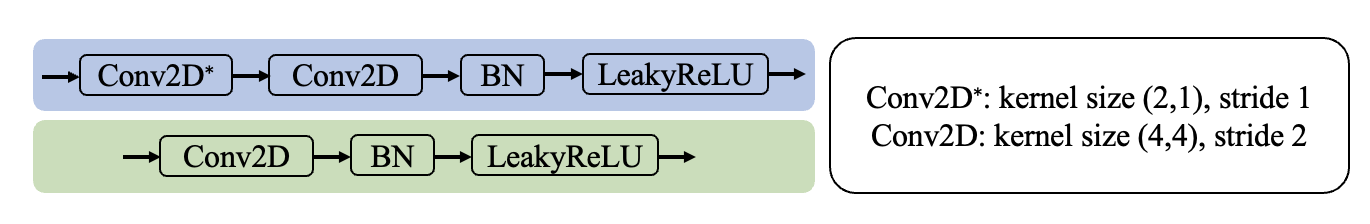
\includegraphics[scale=.62]{thesis/figures/discriminator_downsample.png}
	\caption{Downsample block in the discriminator}
	\label{downsample block in discriminator}
\end{figure}